\documentclass[
	%a4paper, % Use A4 paper size
	letterpaper, % Use US letter paper size
]{jdf}


\author{Nan Xiao}
\email{nanx@gatech.edu}
\title{CS6750 HCI Summer 2021:\\Assignment P2}

\begin{document}
%\lsstyle

\maketitle

\begin{abstract}
	In this paper, we will first discuss 5 tasks in a one-hour period, the goals associated, the interfaces and the objects of interactions. Then for four of these tasks, we will discuss the level of directness and invisibility of the interaction. Second, FIFA video game is discussed as an example of an interface gradually becomes invisible by learning. Third, three types of human perception (visual, auditory, haptic) are discussed for the video game task domain, both existing setups and proposed designs. Also, how taste perception can be used in video games is discussed. Last, we will discuss 2 examples that violating suggestions of reducing cognitive load, and how to redesign those interfaces following the tips.
\end{abstract}

\section{Question1}
\begin{figure}[h]
	\centering
	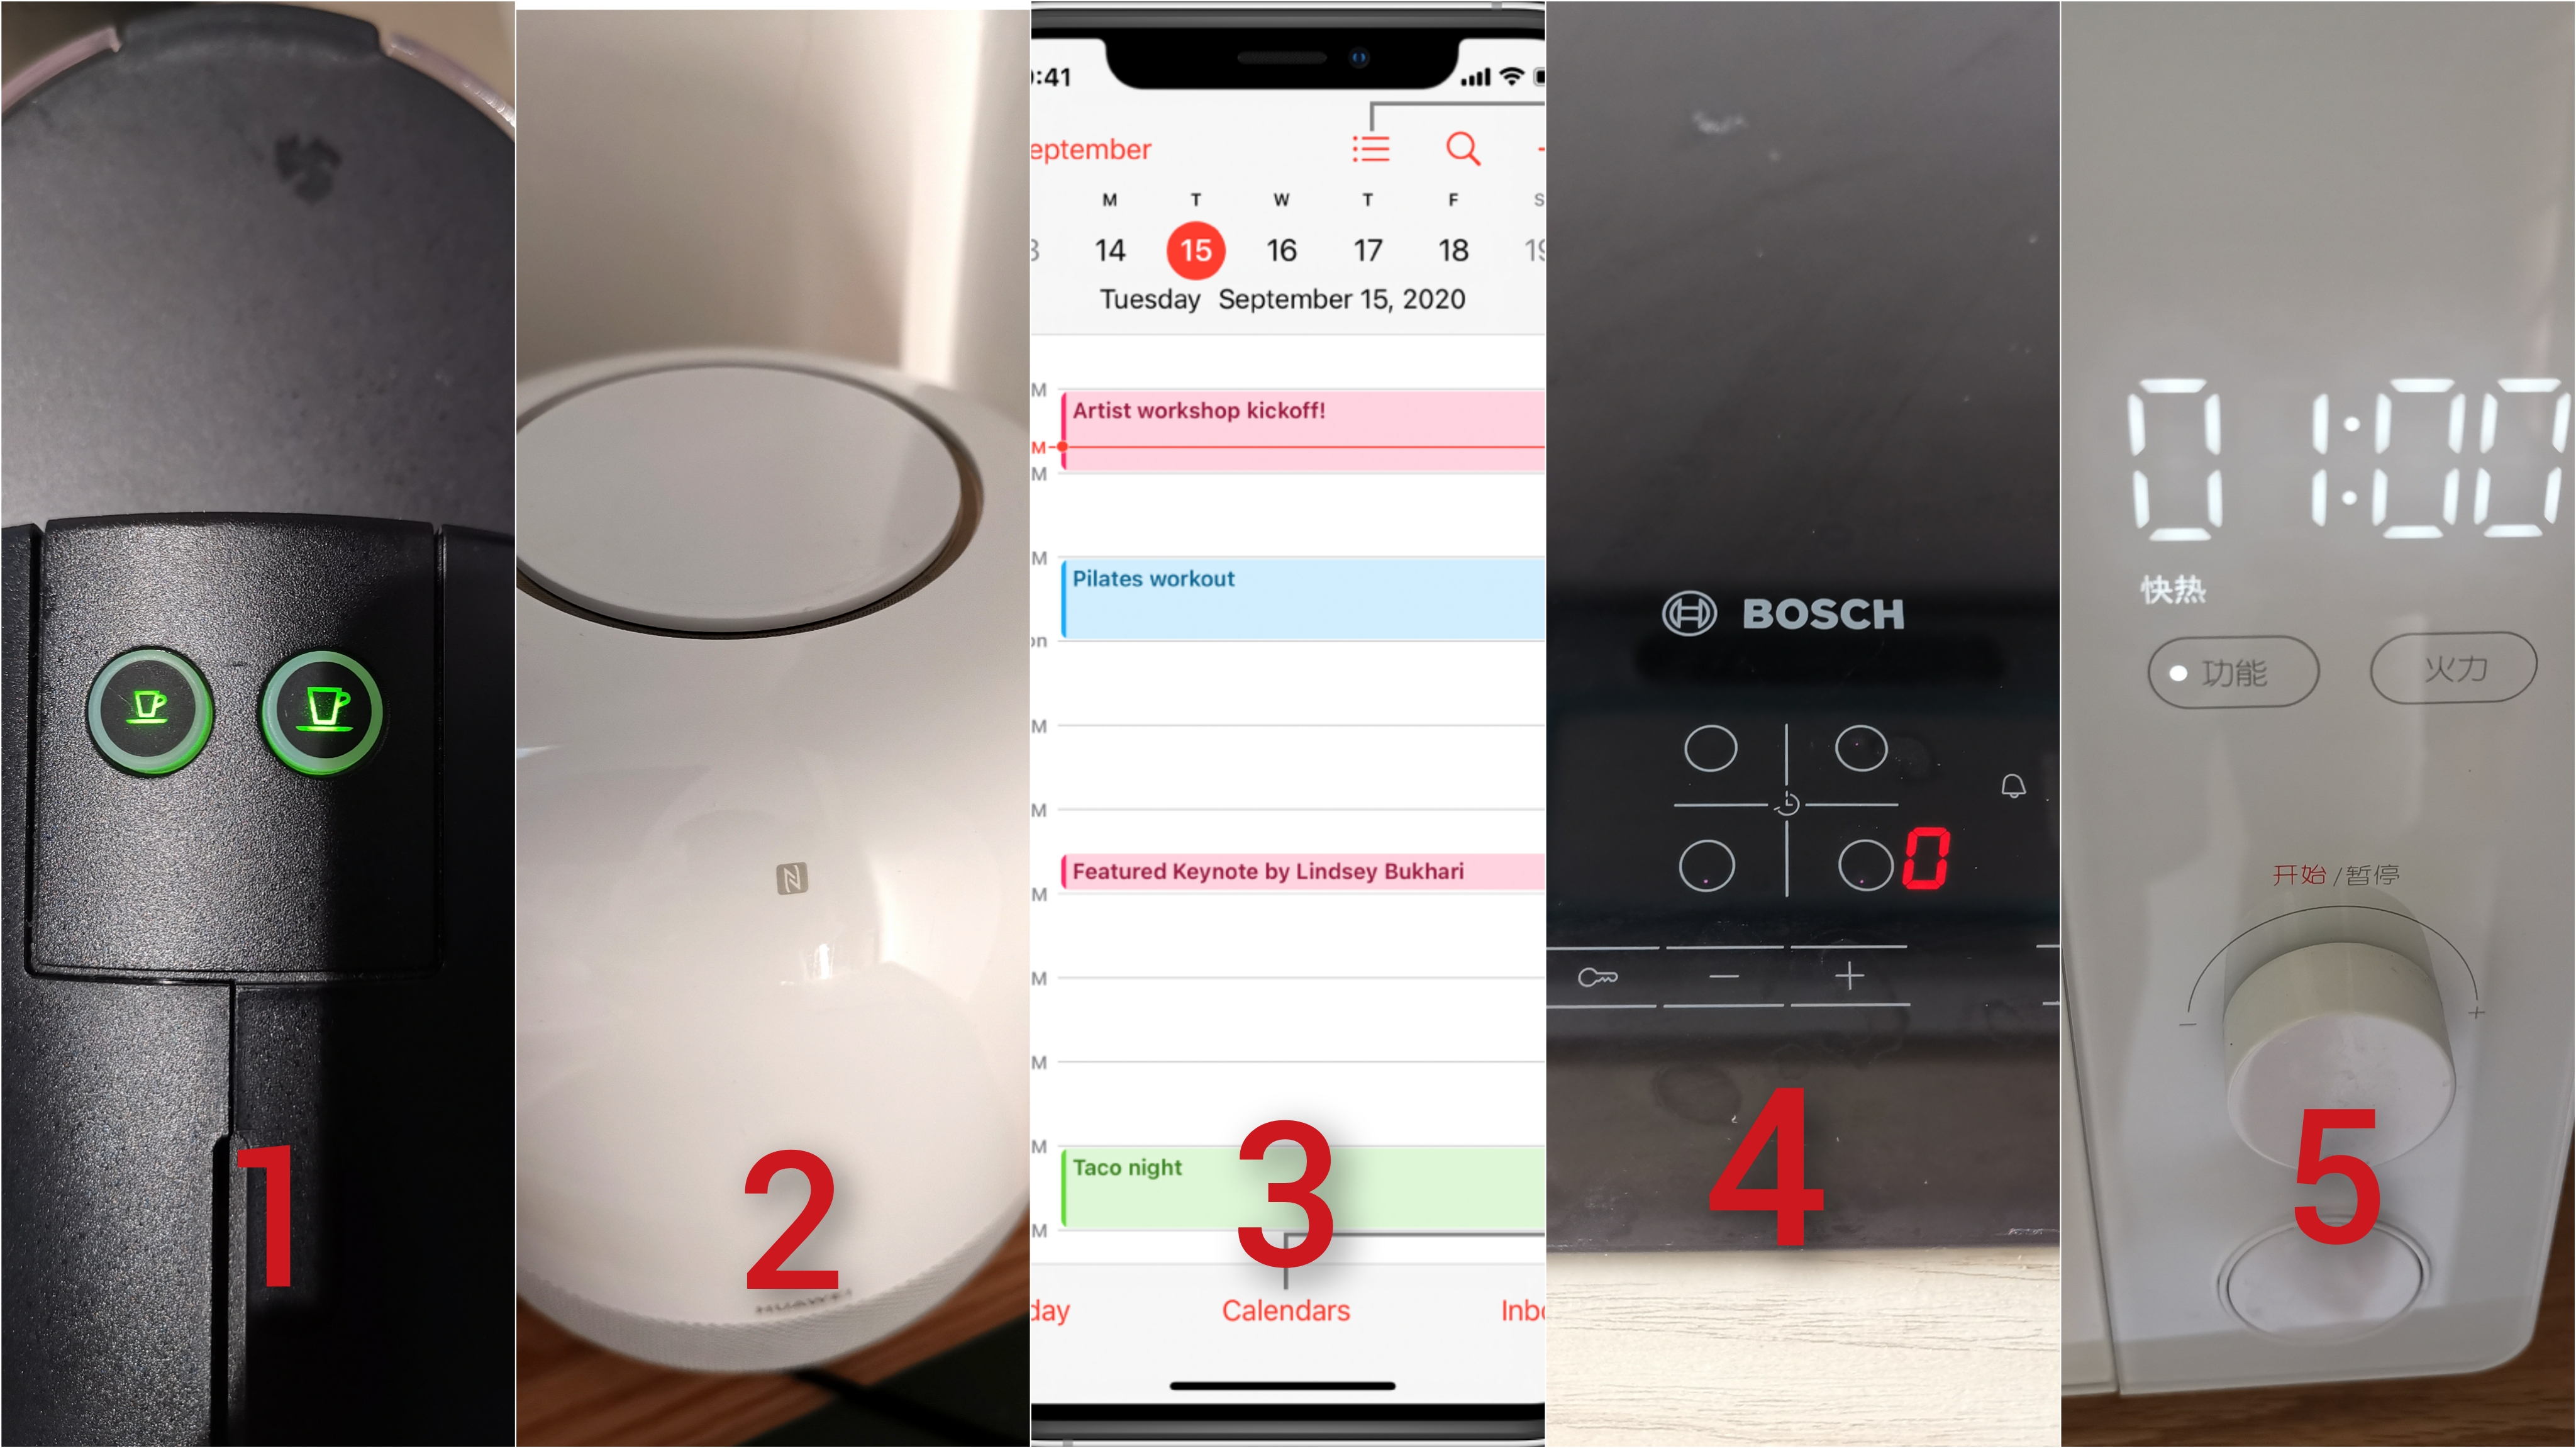
\includegraphics[height=10cm]{jdf-latex/Figures/q1.jpeg}
	\caption{1 - Nespresso machine, 2 - Speaker, 3 - Calendar , 4 - Hob, 5 - Microwave}
	\label{fig:q1}
\end{figure}

\subsection{Table of Five Tasks}
Table 1 contains 5 tasks with their goals, interfaces, and objects.
\begin{table}[h] % [h] forces the table to be output where it is defined in the code (it suppresses floating)
	\caption{Five Tasks with Goals, Interfaces and Objects}
	\small % Reduce font size
	\centering % Centre the table
	\begin{tabular}{L{0.2\linewidth} L{0.2\linewidth} L{0.2\linewidth} L{0.2\linewidth}}
		\textbf{Task} & \textbf{Goal} & \textbf{Interface} & \textbf{Object of interations}\\
		\toprule[0.5pt]
		Use Nespresso machine & Make a cup of coffee & Buttons on Nespresso machine & Coffee capsule\\
		\midrule
		Pair Speaker to Phone & Speaker successfully paired with phone & Screen on Speaker and Phone & Speaker \\
		\midrule
		Add an event to Calendar & Remind me the event at the right time & Calendar app & Phone \\
		\midrule
		Turn on one ring of the induction hob & The correct ring is turned on & Buttons on the hob & Hob \\
		\midrule
		Use microwave to heat the milk & The milk is heated at the right temperature & Buttons on the microwave & Microwave \\
	\end{tabular}
\end{table}


\subsection{Level of Directness & Invisibility of the Interaction}
\subsubsection{Task 1 - Use Nespresso machine}
To make a coffee using Nespresson machine, I need to put the capsule into the machine and press the button twice. My interaction is not directly on the object - coffee capsule, but through the Nespresso machine. The Nespresson machine will then manipulate the capsule to make a cup of coffee. It is not a direct manipulation from the user point of view. Currently I spent most of the time thinking about the task instead of the interface, which is the 2 buttons on the Nespresso machine. But the interface becomes invisible through learning. The first time I use this machine, it took me quite a while to understand you need to press twice the button instead of once to make a coffee.

\subsubsection{Task 2 - Pair Speaker to Phone}
To pair the Huawei speaker to Huawei phone, all I need to do is tap the phone to the speaker. It is incredibly easy and straightforward. My interaction is directly on the object and it is a direct manipulation. I do not spend any time on thinking of the interface. The interface becomes invisible through good design and the user never needs to think about interface. There is a clear logo on the speaker for the user to understand where to tap. And I know the pairing is successful since both screens of the phone and speaker will give feedback.

\subsubsection{Task 3 - Add an event to the phone calendar}
To add an event to the phone calendar, I need to navigate in the calendar app to find the day and time, and then tap to add the event. Doing so I am directly manipulating the object - the calendar app. I spend most of the time thinking about the task rather than the interface, because of the good design that the app looks like a real calendar. Thus the interface becomes invisible and I'm interacting the interface like add a event to the real calendar. It is intuitive for the first-time user as well because of the good design. 

\subsubsection{Task 4 - Turn on one ring of the induction hob}
To turn on one ring of the induction hob, I need to long press the power button, then long press the ring button. I'm directly interacting with the object - the induction hob. I spend less time thinking about the interface now through learning. It used to take me a while to figure out that I need to long press the button instead of short pressing. It is a reasonable design due to safety concern but the first-time user would spend more time on interface instead of the task.

\section{Question2}
\begin{figure}[h]
	\centering
	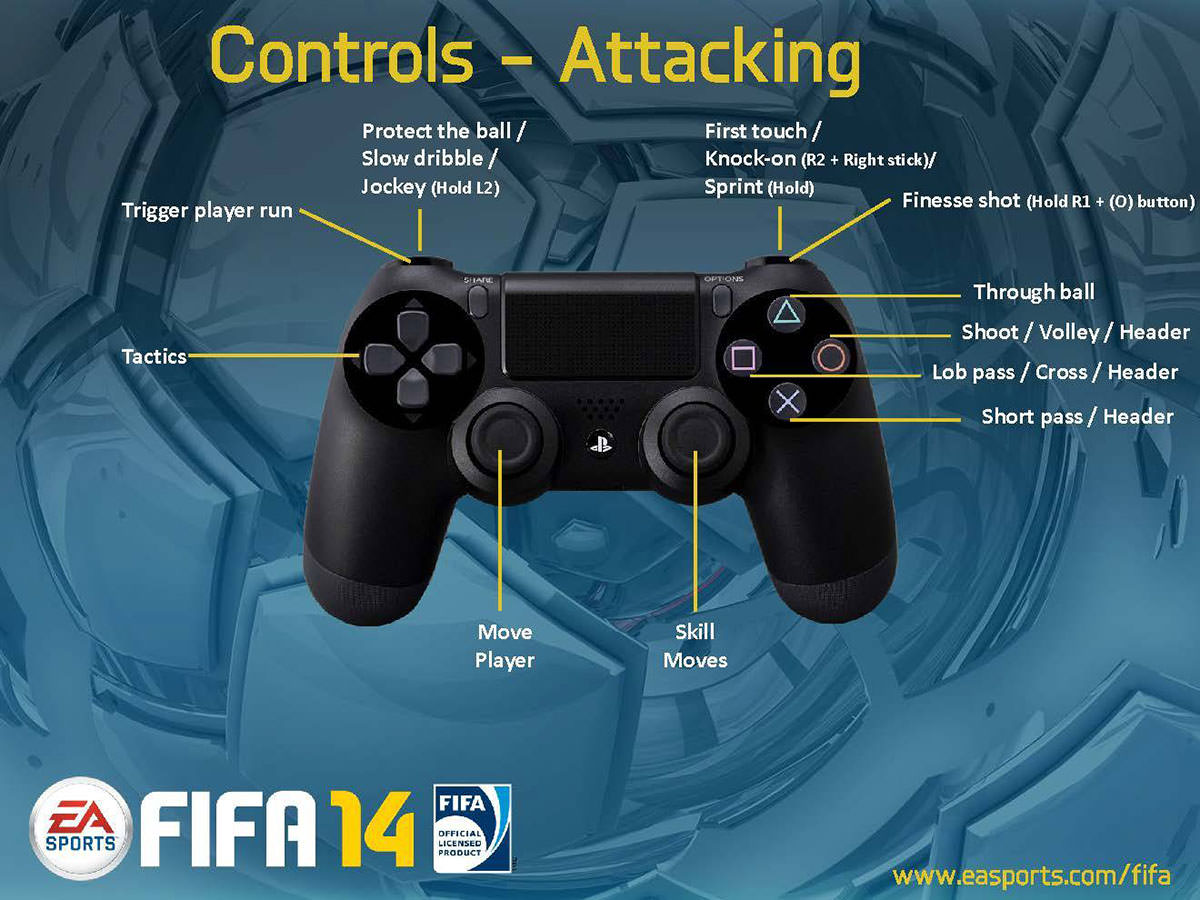
\includegraphics[height=6cm]{jdf-latex/Figures/fifa.jpeg}
	\caption{Complex controls for FIFA}
	\label{fig:fifa}
\end{figure}
In this section, we will study the interface of PS4 controller for FIFA video game. I used to spend a lot of time learning this interface, until it becomes invisible. The interface - PS4 controller consists of many buttons. On the left, there are 4 arrows, normally used for tactics in either attacking of defensing. On the top, there are 4 buttons (R1,R2,L1,L2), normally used combine with 4 shape buttons on the right to perform special movements. The 4 shape buttons on the right are most common actions you would like player to make during attacking and defensing. And on the bottom there are left joystick, which is used for moving players, and right joystick, which is used for skill moves. Both joystick can also be pressed down for different actions. Also, there are 4 extra buttons, "share", "option", "PS button" and "touchpad". "option" can be used to enter menu, and "PS button" can be used to exit game to the PS4 menu. What make the interface more complex is that, when switching from attacking to defensing, most of the buttons are changed for different actions. 

Through hours or days of learning effort by interacting with the controller interface, I eventually build the muscle memory that I understand which buttons to press to make the player do the action as I want it to be. The learning is through manipulation through interface and gather the feedback from the result (player's actual action). When I press the button, the player on the screen will perform an action. With enough learning, I associate the player's action with my muscle memory that I spend most of the time on the task instead of the interface. Even though it takes a lot of time for a user to make interface invisible, the controller is not necessarily a bad design. As a user, I am willing to spend time on learning the interface. Once I spend enough time learning the interface, it becomes invisible. Then I can directly manipulate the object (the player on screen) to do whatever actions with little cognitive effort on the interface.

If I am going to redesign the game, I would like to add another human perception to the interface. Instead of using the controller alone, shooting or passing actions could be assigned to a device monitoring the user's foot movement. It is a more intuitive design to mimic the way people playing soccer. That will reduce the learning curve and offload come cognitive effort to the interface. Then the user can focus more on the task.

\section{Question3}
\begin{figure}[h]
	\centering
	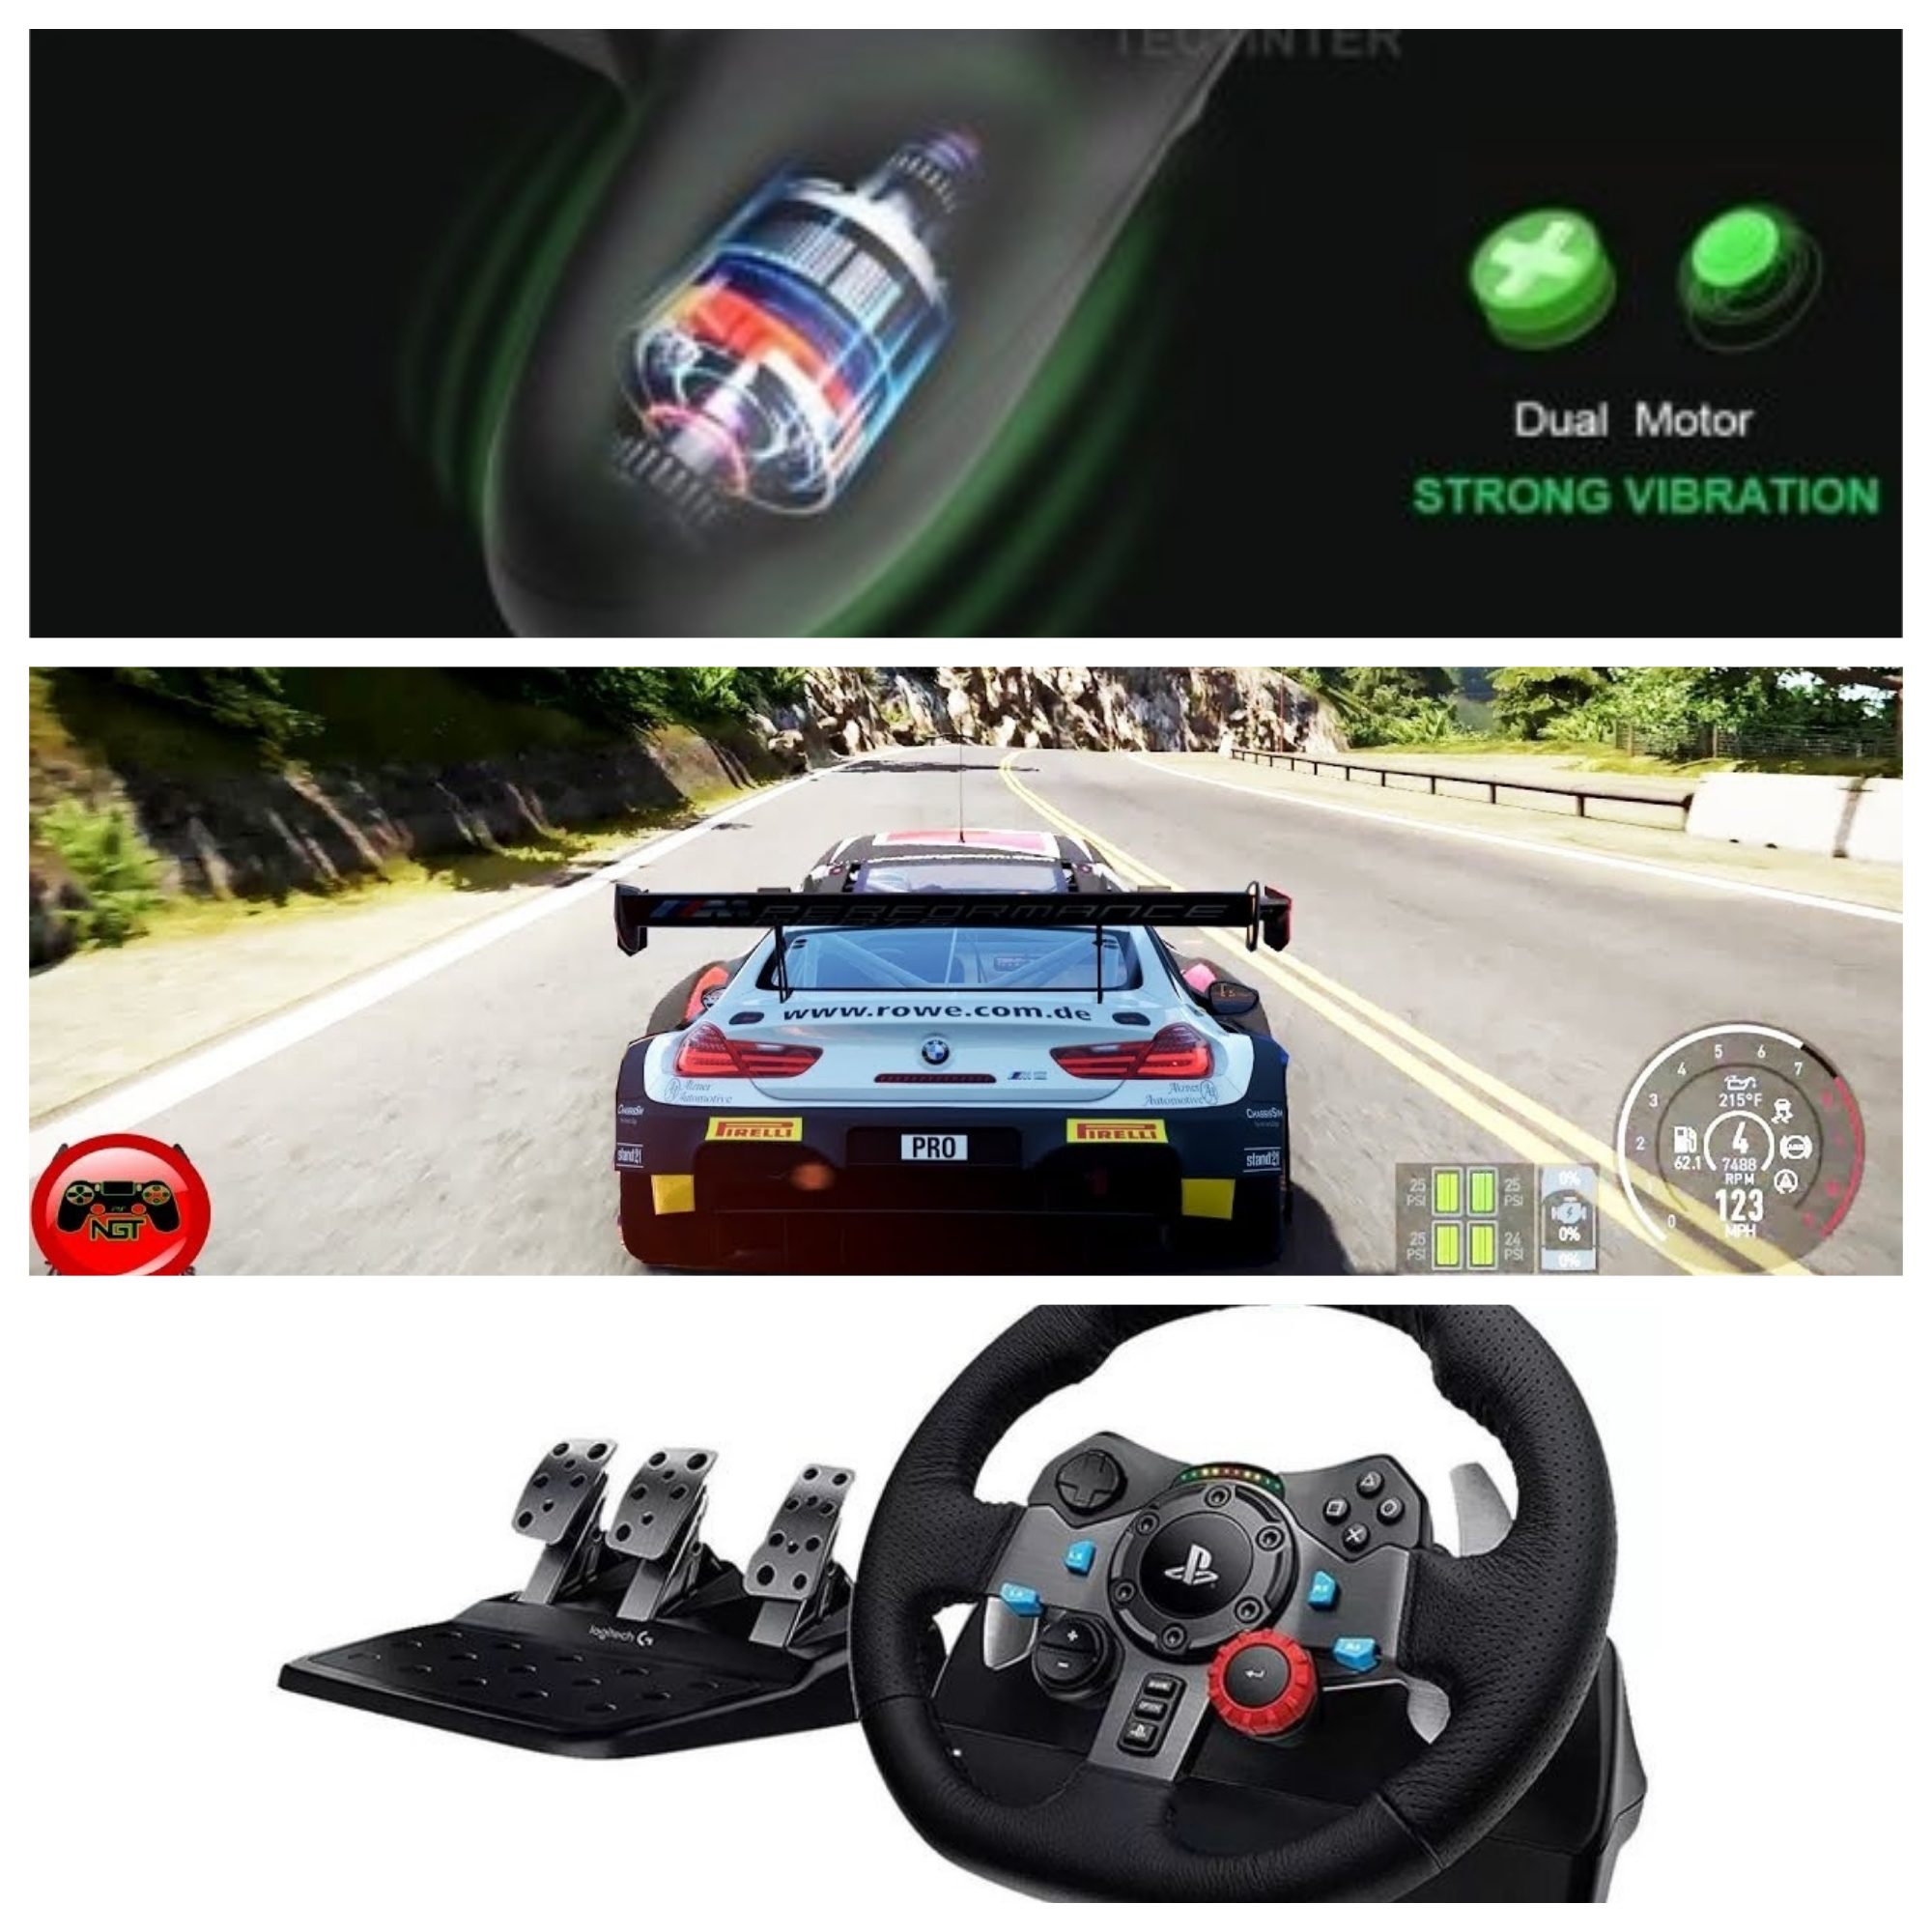
\includegraphics[height=8cm]{jdf-latex/Figures/videogames.jpg}
	\caption{haptic, visual, pressure feedbacks of video games}
	\label{fig:videogames}
\end{figure}
In this section, we will discuss how human perceptions (visual, auditory, haptic) are used to provide feedback in video games. The primary feedback of video game is visual feedback. Players can see the direct impact of their manipulation through the interface (the controller). Take racing video game as an example, when a player move the joystick to the left, the object(car on the screen) will also shift to the left. This direct feedback is easy for the player to understand and evaluate whether his action to the interface generates the desired output. Auditory feedback is used in multiple cases as well. When a rival car is closing, the sound is getting louder from behind to inform the player. Also, when the car collides into other car or the safety fence, a collision sound will inform the player together with a visual feedback. When a car is off the main road, for example driving on the sands, the controller will use the a haptic feedback to inform the player. It is more intuitive for the player to understand he is on the wrong path using haptic feedback, since the car is usually shaky on rough and bumpy road.

Currently, we do not have the visual feedback of how the driver in the car perform when players perform certain actions through the controller. It may be helpful to have that visual feedback that if user move the joystick to the left, not only the car will turn left, but also the driver in the car will steer the wheel to the left. It may offload the cognitive effort if the player has driving experience. The current auditory feedback mainly focuses on the environmental sounds. It would be helpful to add human voice since when a racer racing, he normally has a radio connection with the coaching team. There can be auditory feedback that if player makes a good or bad decision, a radio call will give feedback on that. Haptic feedback is relatively similar due to the technology constrains. With more advanced haptic technology, we may be able to mimic the feedback of acceleration. When a player is speeding up, there would be a stronger acceleration feedback.

Currently, we do not have any feedback from smell perception. This is also due to the technology constrains. There are some popular cooking games like "Overcooked". It would be much better if it can have a smell feedback of the final dish prepared. Also, if small feedback is available, the player can rely on both visual and smell feedback to choose the ingredients. It follows the tips that we should use multiple modalities and they shall complete each other (Joyner, 2021a).

\section{Question4}
Below are the 5 tips of reducing cognitive load (Joyner, 2021a):
\begin{enumerate}
	\item Using multiple modalities
	\item Letting the modalities complement each other
	\item Giving the user control of the pace
	\item Emphasizing essential content while minimizing clutter
	\item Offloading tasks from the user onto the interface
\end{enumerate}
We will discuss 2 examples that violating one of above tips.

\subsection{Internet Banking Transfer Funds}
\begin{figure}[h]
	\centering
	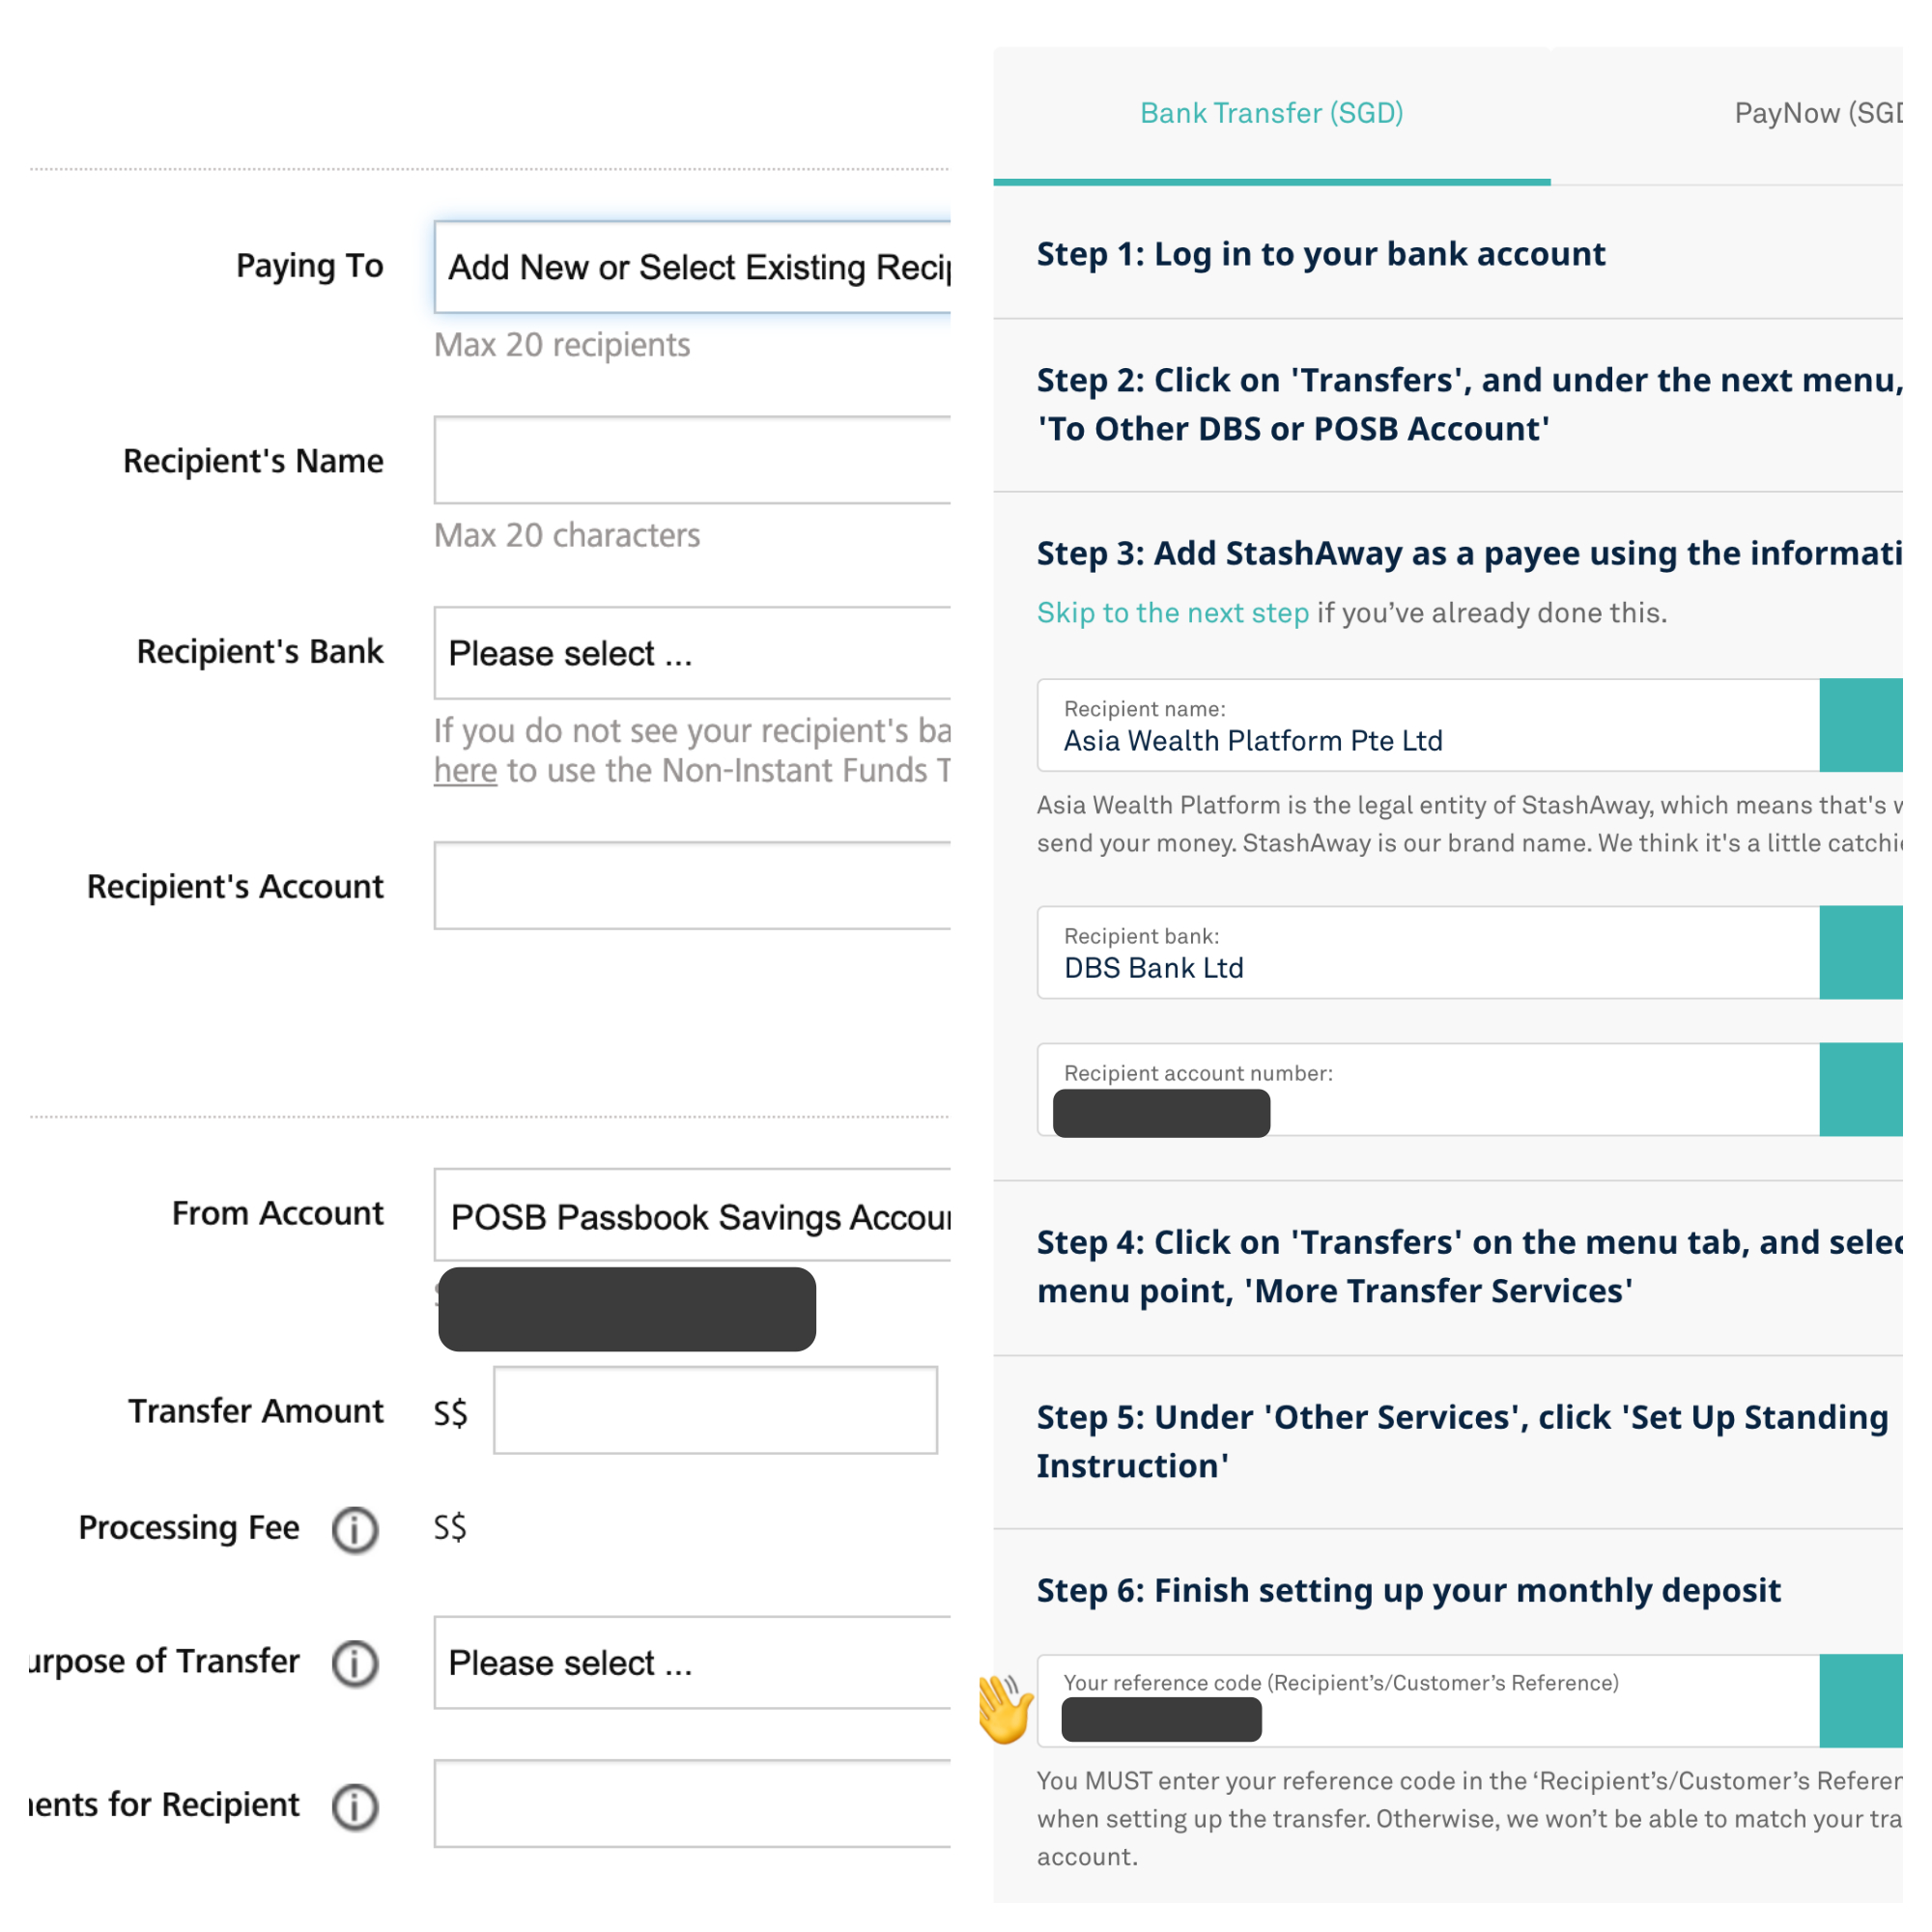
\includegraphics[height=10cm]{jdf-latex/Figures/banktransfer.jpg}
	\caption{Internet banking transfer funds to an investment platform}
	\label{fig:banktransfer}
\end{figure}

To transfer funds using my internet banking, I need to use the interface provided by the bank as shown in the Figure4. To transfer the money, I need to indicate the recipient's name, bank, and account number, and my account, transfer amount, purpose, and comments for recipient. There are 7 items I need to know in order to successfully transfer the money. Plus, it took multiple steps in the internet banking to reach to this page, which is dedicated for the transfer funds task. It is violating the tip that "Offloading tasks from the user onto the interface". Users can only remember "four to five chunks at a time" (Joyner, 2021b). Remembering all the paths to the transfer funds page and 7 items to correctly transfer funds requires too much cognitive load from the users. 

To redesign this task to reduce cognitive load and following the tip, we need to make the interface to take care remember all items other than amount of money to transfer. There should be a button that I can click and it will brings me to the transfer fund page, all I need to key in is the amount of money I would like to transfer. In terms of the security concerns, the interface can initiate a 2FA verification that I need to click "OK" on my phone. This design will reduce most of the cognitive load in this task. 

\subsection{Scan QR Code}
\begin{figure}[h]
	\centering
	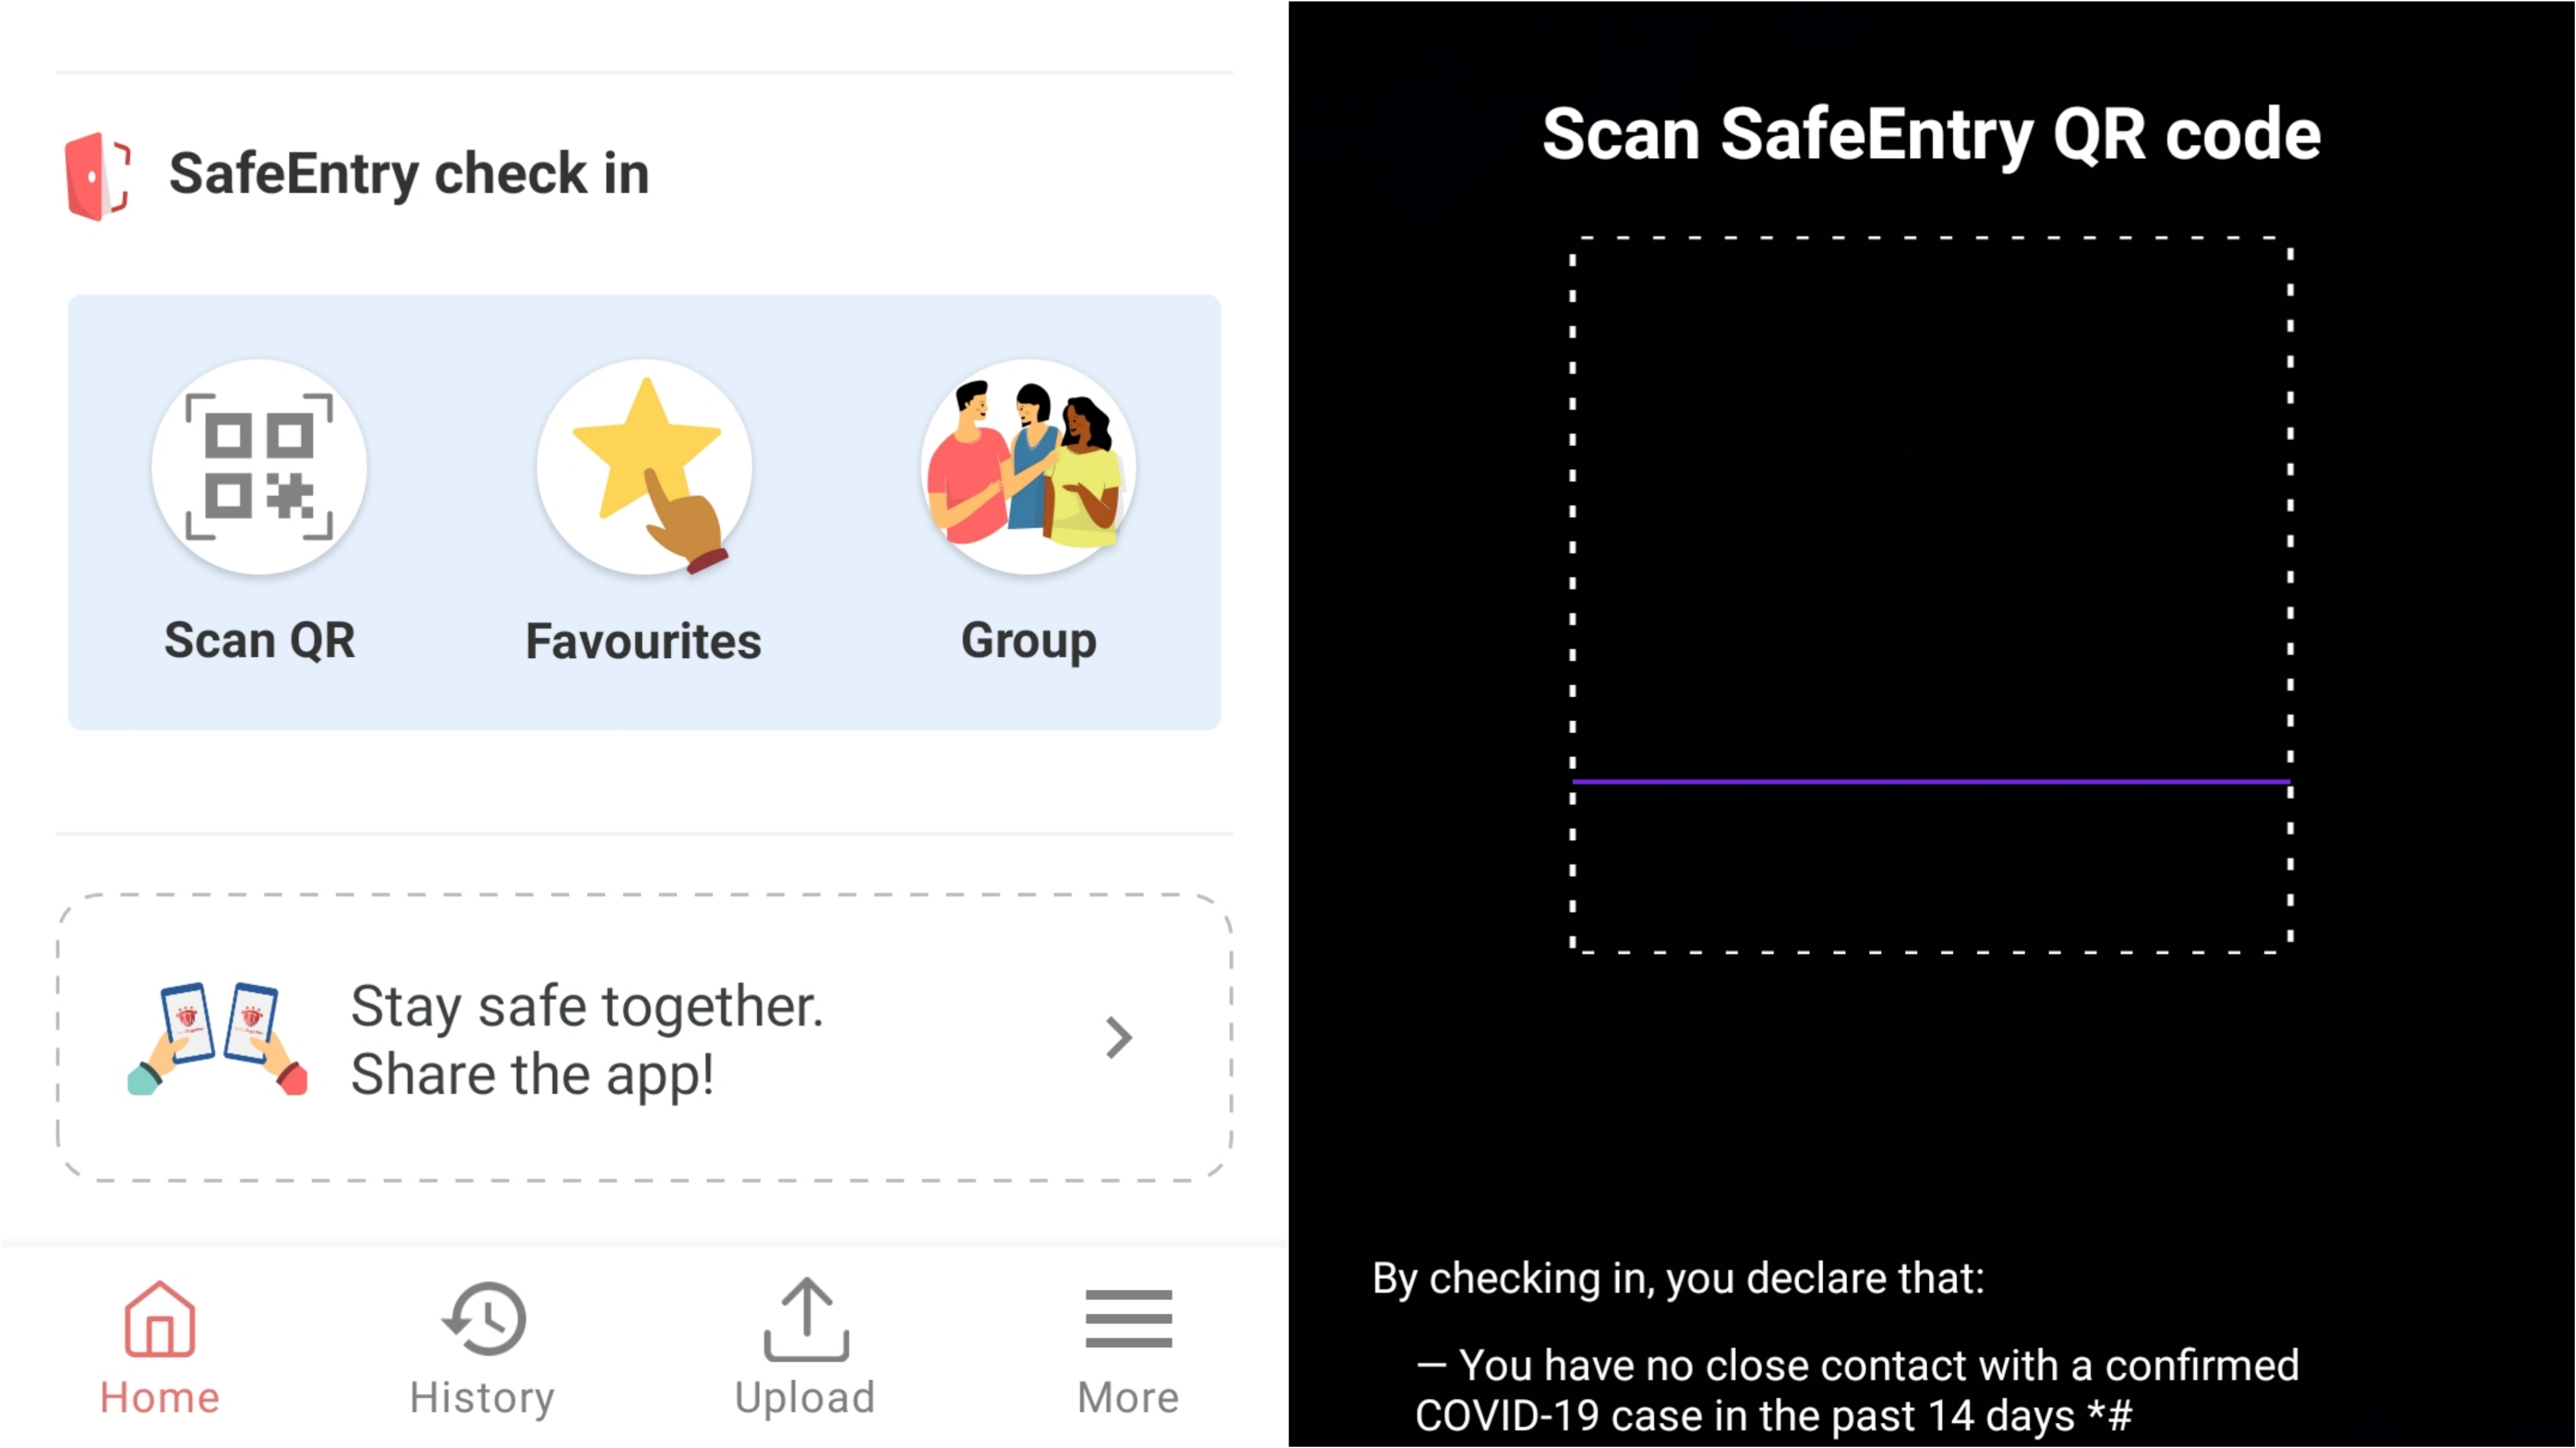
\includegraphics[height=6cm]{jdf-latex/Figures/qr.jpeg}
	\caption{The app to scan QR code}
	\label{fig:qr}
\end{figure}
Since COVID, we need to scan QR code for every place we visit. The interface has a clear button that users can find scanning QR function. Then users need to use the square in the interface to scan the QR code. This interface violates the tip that we should "Use multiple modalities". In the low light case, the task is often failed because the interface is not able to recognize the QR code when the environment does not have enough light. Users would need to turn on the light in this case to make the interface able to scan QR code. It introduces a cognitive load that users need to consider whether the light condition is suitable for the interface to perform well. Thus users spend more cognitive resource on the interface instead of the task. If the interface is able to identify the low-light condition, but without further actions, the user would still need to find extra light for the environment. That would still consume cognitive resources.

The interface should use the sensor to detect the light condition, and turn on the phone's flashlight when low-light environment is detected. It will reduce the user's cognitive load of checking whether light condition is good enough for the interface. Functions like auto-focus, straighten the shape, and remove reflections can all help to reduce the cognitive load of users. Then users can focus on the simple task - scan the QR code instead of worrying about the whether the interface is able to perform.

\section{References}
[1] Joyner, D. (2021a). 5 Tips: Reducing Cognitive Load.

https://classroom.udacity.com/courses/ud400/lessons/

9232968306/concepts/92293480800923

[1] Joyner, D. (2021b). Memory: Short-Term and Chunking.

https://classroom.udacity.com/courses/ud400/lessons/

9232968306/concepts/92293480720923

\end{document}